% !TEX root = ../main.tex
\section{FMT Alignment and Reconstruction} \label{sec::fmtalignmentandreconstruction}
    In paper, the Forwards MicroMegas Tracker (FMT) offers a $3$ to $10$-fold increase in resolution when compared to the Drift Chambers (DC) \cite{aune2009}.
    Achieving this improvement requires work in the alignment and calibration of the detector, and the reconstruction from its data.
    This chapter concerns some of the work done in this endeavour, specifically concerning alignment and reconstruction.

    The first section offers a detailed description of MicroMegas detectors in general and the FMT in particular.
    Then, the second and third sections talk about the efforts done in alignment and reconstruction respectively.
    Finally, the improvement in resolution that results from this work is detailed in the fourth and final section of the chapter.

    % !TEX root = ../main.tex
\subsection{Forwards MicroMegas Tracker}
\label{ssec::forwards_micromegas_tracker}
% --+ Micromegas +--------------------------------------------------------------
    \begin{figure}[b!]
        \centering\frame{
        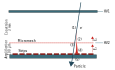
\includegraphics[width=\textwidth]{10mm_principle.pdf}}
        \caption[MM working principle.]{MicroMegas working principle.
        Source: Own elaboration.}
        \label{fig::mm_principle}
    \end{figure}

    A Micro-Mesh Gaseous Detector or MicroMegas (MM) is a gaseous particle detector that follows from the well-known wire chambers.
    These type of detectors are commonly used in experimental physics for the detection of ionising particles.
    The MM detector offers very precise temporal and spatial resolution, to the order of 100 nanoseconds and below 100 micrometers \cite{giomataris1996}.

    The detector works by amplifying the charges that have been created by ionisation in the gas volume.
    It's volume is separated into two parts by a metallic micro-mesh placed less than 150 micrometers of the readouts electrode or strip.

    For clarity, this process is exhibited in figure \ref{fig::mm_principle}.

    While passing through the detector, a particle will ionise the gas atoms by pulling up an electron, creating an electron ion pair (1).
    An electric field is applied to the gas ($\text{E}_1$), allowing the electron to drift toward the amplification electrode (2) and the ion towards the cathode.
    As the electron crosses the mesh (3), it enters an intense electric field ($\text{E}_2$), causing an avalanche effect (4).
    This creates a significant signal at the readout strip (5), which can be then stored for reconstruction \cite{giomataris1996}.

% --+ Micromegas in CLAS12 +----------------------------------------------------
    Inside the CLAS12 detector, a wide array of tracking detectors are used to figure out the positions and momenta of a particle at various points in its trajectory.
    The closer these detectors are to the source of a particle, the more precision is obtained about the position and momentum at the vertex of the interaction, i.e. the point where the particle was produced.
    In an attempt to maximise this precision, the MicroMegas Vertex Tracker (MVT) in CLAS12 is placed as close to the target as possible, as can be seen in figure \ref{fig::mvt}.

    \begin{figure}[b!]
        \centering\frame{
        \includegraphics[scale=0.5]{10mvt.png}}
        \caption[MVT detector.]{MVT detector.
        The red dot denotes the $z=0$ point in the beamline, the red line denotes an arbitrary track coming from that point, and the circumference in the Forward MicroMegas Tracker (FMT) denotes where that track produces a signal in an FMT layer.
        Source: \hyperlink{https://www.jlab.org/physics/hall-b/clas12}{CLAS12 wiki}.}
        \label{fig::mvt}
    \end{figure}

    Just as CLAS12 is divided into a central detector and a forward detector, the MVT is separated into two to maximise the angle coverage:
    The Barrel MicroMegas Tracker (BMT), a barrel tracker made of 18 cylindrical detectors arranged in 6 layers.
    This detector, in combination with the Silicon Vertex Tracker (SVT), covers the region from $35$ to $125\degree$ and greatly improves the polar angle resolution \cite{acker2020mvt}.

% --+ FMT +---------------------------------------------------------------------
    Then, the Forwards MicroMegas Tracker (FMT), which is made of six circular, flat detectors covering angles from $6$ to $29\degree$.
    In theory, it should improve the vertex resolution by a factor of $3$ to $10$ when compared to the Drift Chambers (DC) \cite{aune2009}.
    While the original design of the FMT included six layers, the current implemented detector has only three layers installed.
    This is due to technical difficulties and concerns regarding its Lorentz angle \cite{konczykowski2010}.

    Each of the three FMT layers has $1024$ readout strips, which follow a peculiar distribution, as can be seen in the image to the right of figure \ref{fig::fmt_geometry}.
    In addition, each layer's orientation differs by $60\degree$ to provide an accurate measurement in the xy-plane, as is shown in the image at the centre of the same figure \cite{acker2020mvt}.

    \begin{figure}[t]
        \centering\frame{
        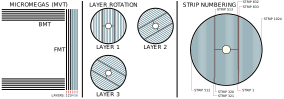
\includegraphics[width=\textwidth]{10fmt_geometry.pdf}}
        \caption[FMT detector geometry.]{FMT detector geometry. The first picture shows the distribution of the BMT and FMT layers, the second the different angle of each FMT layer, and the third the readout strip distribution of each FMT layer.
        Source: Own elaboration.}
        \label{fig::fmt_geometry}
    \end{figure}

\subsubsection{FMT Reconstruction}
    \begin{wrapfigure}{r}{0.50\textwidth}
        \centering\frame{
        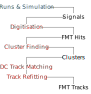
\includegraphics[width=\linewidth]{10fmt_recon.pdf}}
        \caption[FMT reconstruction summary]{FMT reconstruction summary.
        Data taking is coloured blue, data in black, and processes in red.
        Source: Own elaboration.}
        \label{fig::fmt_recon}
    \end{wrapfigure}

    After a signal is detected on a readout strip and the data is stored, information is obtained from it from offline reconstruction.
    Being a tracker, FMT's reconstruction works in a fairly similar manner to DC's.

    First, after a signal is detected in a strip it is digitised, processed, and turned into an \textbf{FMT Hit}.
    A group of FMT hits is processed via a \textbf{Cluster Finding} algorithm, where a \textbf{Cluster} is defined as a group of hits that supposedly come from the same particle track.
    A group of clusters from different layers go through a \textbf{DC Track Matching} algorithm, where they are matched to DC tracks from DC Reconstruction.
    A \textbf{Track Refitting} algorithm is applied for each DC track using the clusters' data, updating them to re-fitted tracks, named \textbf{FMT tracks}.
    This whole process is summarised in figure \ref{fig::fmt_recon}.

\clearpage

    % !TEX root = ../main.tex
\subsection{FMT Alignment} \label{ssec::fmtalignment}
% --+ Why is it needed +--------------------------------------------------------
    While in a perfect world the target and each detector would be installed precisely where they are needed, in the real world there is an unavoidable misalignment in their positions.
    This misalignment needs to be addressed and included into reconstruction:
    the software needs to be aware of where a detector is positioned in relation to the target to provide meaningful results.

    In the CLAS collaboration, the Calibration and Commissioning group (CalCom) is in charge of the alignment and calibration of each detector.
    Shifts and rotations that need to be applied for alignment are included in the Calibration and Conditions Database (CCDB), which is then read in reconstruction. % NOTE. A citation would be cool.

    The main goals of alignment work were three:
    First, to provide FMT alignment tables to Run Group F (RG-F) so that they may be used in reconstruction.
    Second, to check if the resolution improvement from FMT is good enough to justify the extra material added to the CLAS12 detector.
    Finally, to provide detailed information about these improvements so that Run Group E (RG-E) and other run groups can choose if they will include the detector to their runs.

% --+ Definitions +-------------------------------------------------------------
    Alignment shifts can be made in any of the three global axes:
    $z$, which is concentric to the beamline, $x$, which is parallel to the ground, and $y$, which points up from the ground.
    Then, alignment rotations can be done in any of these axes, and for the purposes of this work will be referred to as $\phi$ rotation (roll), when they're done around the $z$ axis, and pitch and yaw when they're done around the $x$ and $y$ axes respectively.

    To measure misalignment, we define a the Distance Of Closest Approach (DOCA) between a reconstructed DC track and an FMT cluster as a \textbf{Residual}.
    Due to each layer's geometry (refer to figure \ref{fig::fmt_geometry}), only the residuals in a layer's local $y$ axis (perpendicular to the strips) can be measured.
    This means that global $z$ and $\phi$ alignment can be done for each layer independently, but global $x$, global $y$, pitch, and yaw alignment has to be done for the entire detector at once.

% --+ How was it done +---------------------------------------------------------
    \begin{figure}[b!]
        \centering\frame{
        \includegraphics[width=\textwidth]{12fmtalign/img/20res_example.png}}
        \caption{Example residuals plot.}
        \label{fig::res_example}
    \end{figure}

    To minimise residuals, they are plotted for a particular shift or rotation in any of the relevant axes.
    An example of such a plot is shown in figure \ref{fig::res_example}.
    Since a Gaussian distribution is to be expected for the residuals, a Gaussian fit is applied to them.
    For $z$ and $\phi$ alignment, the goodness of a fit is evaluated heuristically by comparing their $\sigma$ and choosing the shift with the minimum $\sigma$.
    Then, for $x$, $y$, pitch, and yaw alignment, the goodness of a fit is evaluated heuristically by choosing the fit with the mean closest to $0$.
    The minimums are of course chosen within a healthy error margin.
    Examples of $z$ and $xy$ goodness of fit distributions can be seen in figure \ref{fig::resfit_example}.

    \begin{figure}[t!]
        \centering\frame{
        \includegraphics[width=\textwidth]{12fmtalign/img/20resfit_example.png}}
        \caption{Examples of residuals goodness of fit plots.}
        \label{fig::resfit_example}
    \end{figure}

% --+ Cuts +--------------------------------------------------------------------
\subsubsection{Fiducial Cuts}
    To reduce background, fiducial cuts are applied to the DC tracks and FMT clusters.
    This process is useful to increase data quality in order to obtain meaningful alignment results.

    For DC tracks, the cuts applied are:
    \begin{itemize}
        \item $\text{track}.z < \text{layer}.z$:
        Remove tracks with a vertex $z$ further downstream than the FMT layer before swimming.
        This is caused by reconstruction errors where the particle origin is outside of the target.
        % $9.84\%$ of tracks fail to meet this criterion in the sample data.
        \item $\mid\text{track}.z - \text{layer}.z\mid < 0.05 \text{cm}$:
        Remove tracks too far from the FMT layer after swimming.
        This was caused by bugs in the swimmer which will be mentioned in the next section.
        % $18.67\%$ tracks failed to meet this criterion.
        \item $5 \text{cm} < \sqrt{x^2 + y^2} < 25 \text{cm}$:
        Remove tracks outside of the layer's active region.
        % $35.22\%$ of the tracks were lost to this criterion.
        \item $\theta < ~66.42^{\circ}$:
        Remove tracks with a $\theta$ angle too high.
        When this happens, the same particle is affecting many strips, which causes the detector's data to not be as reliable as we want for alignment.
        % $7.22\%$ of tracks were lost to this criterion.
    \end{itemize}
    % From all these criteria, $70.95\%$ of the DC tracks were lost.
    % It is worth noting that after some reconstruction errors were fixed (as will be detailed in the following section), this percentage was reduced to $52.28\%$.

    For FMT clusters, the cuts applied are:
    \begin{itemize}
        \item $50 \text{ns} < \text{T}_{\text{min}} < 500 \text{ns}$:
        Cut clusters with an illogical $\text{T}_{\text{min}}$, which is the time of the first hit in the cluster.
        % $21.12\%$ of clusters fail to meet this criterion.
        \item $\text{size} > 1$ $\&\&$ $\text{E} > 100$:
        Cut small clusters with high energy, which are generally considered bad.
        % Only $7.36\%$ clusters are lost to this criterion.
        \item $\text{size} < 5$:
        Cut large clusters, which are not considered very useful.
        % Only $7.77\%$ are lost to this criterion.
    \end{itemize}
    % From all these criteria, $36.25\%$ of the FMT clusters were lost.

% --+ Minimisation of residuals +-----------------------------------------------
\subsubsection{Residuals Improvements}
    To validate the alignment algorithm proposed, it was tested on RG-F data (run $\mathbf{11983}$).
    The improvement in residuals is immediately obvious, as can be seen in figure \ref{fig::res_comparison}, noting the difference in scale between the top and bottom plots.

    \begin{figure}[t!]
        \centering\frame{
        \includegraphics[width=\textwidth]{12fmtalign/img/20res_comparison.png}}
        \caption[Residuals distribution improvement.]{Residuals distribution before (upper image) and after (lower image) alignment.}
        \label{fig::res_comparison}
    \end{figure}

    As can be seen in the figure, the $z$ and $\phi$ alignment heavily reduces the background, increasing the number of residuals near the mean of the distribution.
    In addition, the $x$ and $y$ alignment pushes this mean to zero, whereas it was slightly off before.
    Finally, no meaningful results were obtained for pitch and yaw alignment.
    This is attributed to how small the rotations around the $x$ and $y$ axes are, compounded with the fact that three layers do not provide enough data to perform alignment precise enough.

    To measure the mean and $\sigma$ of the distribution, a Gaussian fit was used.
    Its parameters are

     \begin{align*}
        \Big( \text{amp} \cdot \text{gaus}(\mu, \sigma) \Big) &+ \Big( p_0 + p_1\cdot x + p_2\cdot x^2 \Big) \\
        \text{gaussian} \hspace{0.8cm} &+ \hspace{1cm} \text{background}
    \end{align*}

    The results obtained are included in the CCDB at:

    \small\href{https://clasweb.jlab.org/cgi-bin/ccdb/versions?table=/geometry/fmt/alignment}{\texttt{clasweb.jlab.org/cgi-bin/ccdb/versions?table=/geometry/fmt/alignment}}

    Alignment was also later performed for Run Group M (RG-M) data successfully, proving that the alignment procedure is agnostic to a particular run.
    How this alignment procedure affects the resolution of the entire CLAS12 detector will be explored at the end of the chapter.

    The procedure described in this section is documented and shared publicly.
    It can be seen at:

    \href{https://github.com/JeffersonLab/clas12alignment/tree/master/fmt}{\texttt{github.com/JeffersonLab/clas12alignment/tree/master/fmt}}

    % !TEX root = ../main.tex
\subsection{FMT Reconstruction} \label{ssec::fmtreconstruction}
% --+ Why is it needed +--------------------------------------------------------
    As work in FMT alignment progressed, some changes were needed in FMT reconstruction.
    These changes mainly include the implementation of the shifts found in alignment to reconstruction.
    However, they also concern some fixes of issues found as alignment work progressed.

% --+ What was done +-----------------------------------------------------------
    First, the loading of shifts from the CCDB was included in the standard geometry class of the FMT reconstruction package.
    Then, standard methods to include the shifts in any frame of reference change were included.
    Finally, the code was studied in detail and the shits were added in all instance where they were required, since the package originally didn't consider their application.

    ``Crossmaking'' is the process of matching clusters in different layers to obtain an accurate 3D estimate of the position of a track \cite{ziegler2020}.
    This was originally included in FMT reconstruction to facilitate reconstruction for the six FMT layers.
    However, as was mentioned before, only three FMT layers were installed for the RG-F run, and future runs may also use three layers due to concerns with the Lorentz angle if six are used.
    To simplify reconstruction and make better use of this number of layers, crossmaking was removed from reconstruction.

    Outside of FMT reconstruction, some minor changes were also required in the DC reconstruction package, since some of its components depends on the FMT layers' positions.
    In addition, the swim package diagnostic was updated, since it failed to properly reconstruction the positions of tracks near the FMT layers.

% --+ Juicy link +--------------------------------------------------------------
    A detailed list of the updates applied can be found in the following pull request to the \texttt{clas12-offline-software} repository:

    \href{https://github.com/JeffersonLab/clas12-offline-software/pull/726}{\texttt{github.com/JeffersonLab/clas12-offline-software/pull/726}}.

    % !TEX root = ../main.tex
\subsection{Validation and Results} \label{ssec::validationandresults}
% --+ Data used +---------------------------------------------------------------
    Just as with the residuals validation, the results presented in this document are based on the application of this work on RG-F data.
    It's worth noting that the RG-F target is $\sim60$ centimetres long, much larger than the average CLAS12 target \cite{hattawy2019}.
    In particular, the runs used for testing and validation are presented in table \ref{tab::rgf_data}, and the run used to obtain the data displayed in this section was $\mathbf{011983}$.

    \begin{table}[h!]
        \centering
        \begin{tabular}{c|llll}
            \textbf{Run Number} & \textbf{Energy (MeV)} & \textbf{Current (nA)} & \textbf{Configuration} & \textbf{Target} \\
            \hline
            \textbf{011983}     & 10389.4 &  50 & Inbending & D2 \\
            \textbf{012016}     & 10389.4 & 250 & Inbending & D2 \\
            \textbf{012439}     &  2186.4 &  15 & Inbending & H2 \\
            \textbf{012461}     & 10196.6 &  20 & Inbending & D2
        \end{tabular}
        \caption{RG-F runs used for validation.}
        \label{tab::rgf_data}
    \end{table}

% --+ Cuts +--------------------------------------------------------------------
    Some additional cuts are applied to the tracks to obtain the plots presented in this section.
    These cuts are merely to remove very bad tracks which would nonetheless not be used in analysis.
    \begin{itemize}
        \item \texttt{abs(chi2pid) < 5}: Remove tracks without enough certainty on the PID of a particle.
        \item \texttt{vz < fmtZ}: Remove tracks further downstream than FMT.
        \item \texttt{chi2/ndf < 15}: Don't use tracks with too much uncertainty.
    \end{itemize}

% --+ Geometry issue +----------------------------------------------------------
    To measure the improvement in vertex resolution, we'll compare the vertex position of tracks that passed only through DC reconstruction and tracks that passed through both DC and FMT reconstruction.
    For simplicity, we'll refer to the former as DC tracks and the latter as FMT tracks.
    Remembering that the $z$ axis is concentric with the beamline, figure \ref{fig::dc_vs_fmt_vz} shows the vertex $z$ position of DC tracks versus that of FMT tracks.

    \begin{figure}[h!]
        \centering\frame{
        \includegraphics[width=\textwidth]{12fmtalign/img/40dc_vs_fmt.png}}
        \caption[DC vs FMT $z$ without geometric correction]{DC vs FMT vertex $z$ for electrons without any geometric correction. DC tracks are shown in green while FMT tracks are shown in blue. Note that the dark cyan colour comes from the overlap.}
        \label{fig::dc_vs_fmt_vz}
    \end{figure}

    To understand the plot in the figure, it's worthwhile to take a minute to look at the RG-F target.
    The target itself is a large chamber filled with gas, with a composition that changes across runs.
    The distance between the windows of the chamber is of $553.32$ millimetres.
    In addition, it was found that the upstream window of the target is separated by about $24$ millimetres from the beam window.
    % This is a far cry from the nominal distance, which was expected to be of $9.16$ millimetres.
    All windows are made of aluminium and have a thickness of $15$ micrometres. % TODO. CITATION PENDING.
    A detailed drawing of the target can be seen in addendum 1.

    From figure \ref{fig::dc_vs_fmt_vz}, it is immediately obvious that the FMT detector only recognises the upstream windows, completely missing the downstream one.
    This is purely a geometric issue:
    the downstream window is outside of the FMT active detection area.
    The effect is easy to see in figure \ref{fig::vz_vs_theta}, where the vertex $z$ coordinate is plotted against the $\theta$ angle.
    The two red lines in the plots show FMT's active area, and the downstream windows is clearly outside of it, hence why it disappears.

    \begin{figure}[t!]
        \centering\frame{
        \includegraphics[scale=0.24]{12fmtalign/img/40theta_dc_vs_fmt.png}}
        \caption[$z$ vs $\theta$ for DC and FMT.]{$z$ vs $\theta$ for DC and FMT for electrons without any geometry correction. FMT's active area are shown in red lines.}
        \label{fig::vz_vs_theta}
    \end{figure}

    To account for this geometric effect, we apply an additional cut based on the plotted curves.
    The curves are given by
    \begin{equation*}
        c_1 = 57.29 \cdot \arctan\left(\frac{r_\text{inner}}{z_0 - z}\right), \hspace{0.5cm}
        c_2 = 57.29 \cdot \arctan\left(\frac{r_\text{outer}}{z_0 - z}\right),
    \end{equation*}
    where $r_\text{inner}$ is the radius of the hole at the center of FMT, $r_\text{outer}$ is the radius of the outer circumference of FMT, and $z_0$ is the $z$ position of the first FMT layer plus the drift distance.
    All these parameters are read from the CCDB.

% --+ Show vertex position resolution improvement +-----------------------------
    In addition, one final cut was added.
    At the time of writing, beam alignment is yet to be performed for RG-F data, which causes a loss in vertex resolution.
    Since this hampers the accuracy of reconstruction, we added an additional cut to only use one sector of the detector.

    \begin{figure}[b!]
        \centering\frame{
        \includegraphics[scale=0.24]{12fmtalign/img/40dc_vs_fmt_sector1.png}}
        \caption[DC vs FMT $z$ with geometry correction]{DC vs FMT vertex $z$ for electrons with a geometric correction. DC tracks are shown in green while FMT tracks are shown in blue. Data from only one CLAS12 sector was used to obtain this plot.}
        \label{fig::dc_vs_fmt_vz_corrected}
    \end{figure}

    The resolution plot contrasting DC and FMT tracks using all the cuts referred up to this point can be seen in figure \ref{fig::dc_vs_fmt_vz_corrected}.
    To measure both DC and FMT resolution, we'll use two Gaussian curves compounded with a quadratic curve to account for the background.
    The fit is defined as
    \begin{equation*}
        \text{amp}_1 \cdot \text{gaus}(z, z_\text{max}, \sigma) + \text{amp}_2 \cdot \text{gaus}(z, z_\text{max} - 2.4, \sigma) + p_1 + p_2\cdot z + p_3\cdot z^2,
    \end{equation*}
    where $\text{amp}_1$ is the amplitude of the biggest peak and $z_\text{max}$ is its $z$ position, $\text{amp}_2$ is the amplitude of the leftward peak, whose position was measured to be $2.4$ centimetres, and all the other parameters are obtained by fitting.

% --+ Resolution for electrons +------------------------------------------------
    % TODO. Update with plots from rge-analysis.
    For electrons in run \textbf{011983} (low luminosity, $50$ nA), this gives a DC resolution of $\sigma_\text{DC} = 0.875$ cm and an FMT resolution of $\sigma_\text{FMT} = 0.387$ cm --- a doubling in resolution.
    For electrons in run \textbf{012016} (production luminosity, $250$ nA), this gives a DC resolution of $\sigma_\text{DC} = 1.009$ cm and an FMT resolution of $\sigma_\text{FMT} = 0.596$ cm.

% --+ Resolution with no particle cuts +----------------------------------------
    % TODO. Update with plots from rge-analysis.

% --+ Conclusions +-------------------------------------------------------------
    While the improvement in resolution is less than what was originally predicted for the detector, it is still a very encouraging result.
    The increase in resolution allows for more precise target position measurements.
    This, for example, allows for double targets to be placed closer to each other, benefiting the physics derived from such experiments, such as the RG-E run. % TODO. CITATION NEEDED.

    The reason behind the improvement not being as large as predicted is attributed to the fact that the original projection considered six FMT layers.
    This amount of layers would add more position data in the particle's track, allowing the fitting process to better measure its vertex position.

% --+ Why no improvements is seen on vertex momentum resolution +---------------
    In addition, the lack of more layers and the proximity between them means that FMT has a small lever arm.
    This means that the detector cannot provide a good contribution to the vertex momentum resolution, since there is not enough data added to the track's momentum. % TODO. MAYBE CITATION NEEDED?

% --+ Show detector efficiency +------------------------------------------------
    Finally, in the interest of understanding the FMT detector, we briefly study the efficiency of FMT.
    We define efficiency as the number of FMT tracks divided by the number of DC tracks or, in other words, how many of the DC tracks were detected by FMT as well.
    With the three layer configuration, efficiency is $\sim 88.96\%$.
    As can be seen in figure \ref{fig::fmt_efficiency}, there is no anomalous geometric effect in layer-by-layer efficiency.
    The gaps seen are merely due to the geometry of CLAS12, since its separated into six sectors.

    \begin{figure}[b]
        \centering\frame{
        \includegraphics[width=\textwidth]{12fmtalign/img/40fmt_efficiency.png}}
        \caption[FMT layers efficiency]{Efficiency of each FMT layer.}
        \label{fig::fmt_efficiency}
    \end{figure}

